

\section{二原子分子の振動・回転遷移}
\begin{figure}[]
 \begin{center}
	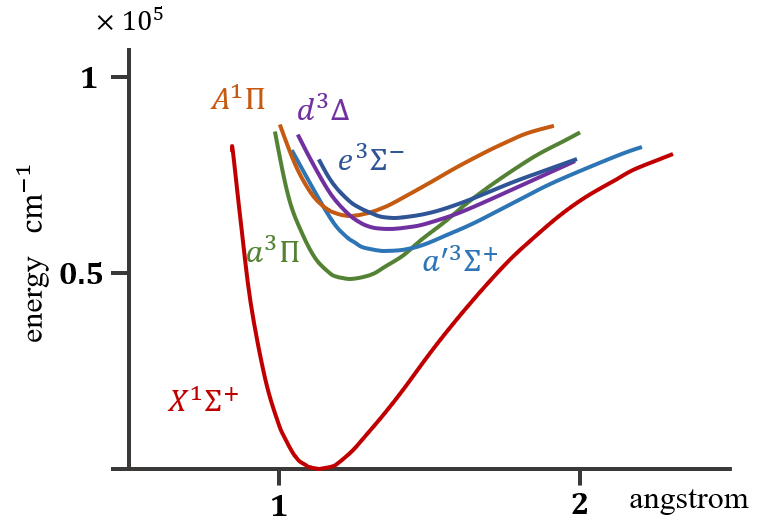
\includegraphics[width=1.0\linewidth]{fig/co_ele_state.png}
% 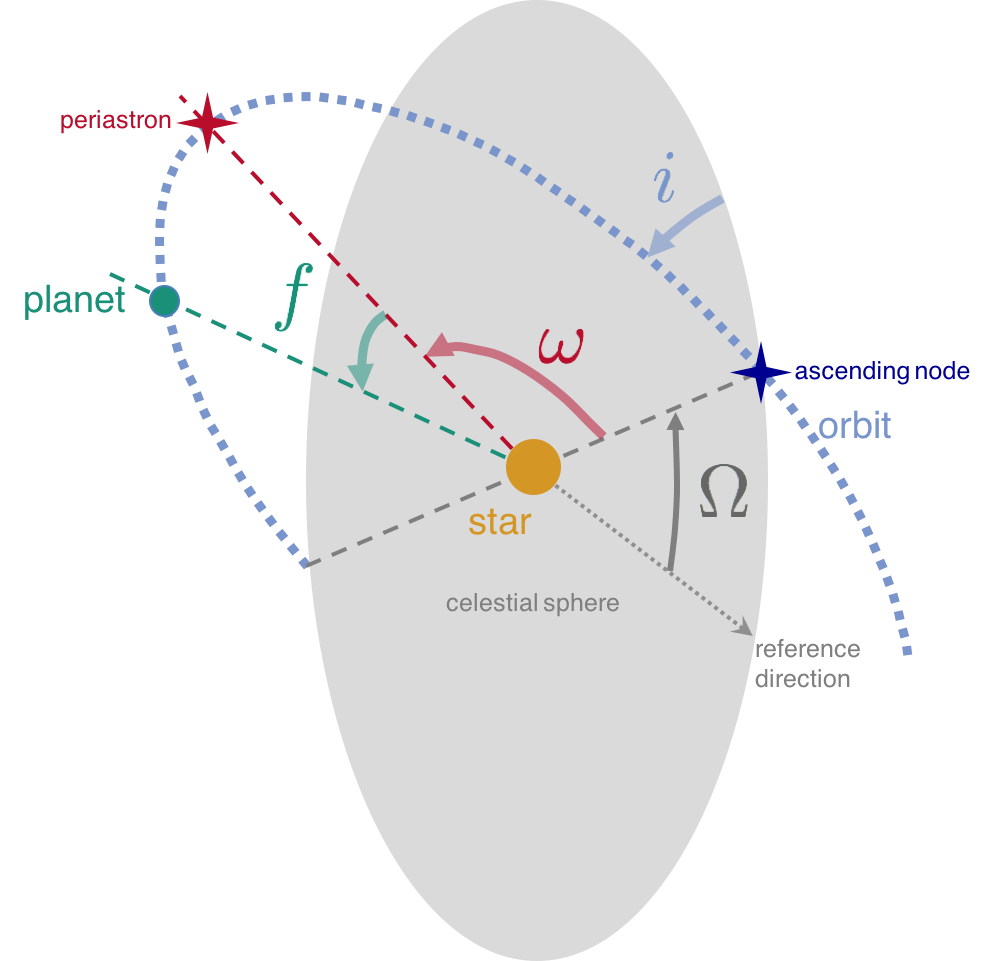
\includegraphics[bb=0 0 474 461,width=1.0\linewidth]{fig/orbele.png}
\end{center}
	\caption{一酸化炭素の電子状態。横軸は核子(炭素-酸素)間距離。}
	\label{fig:co_ele_state}
\end{figure} 

二原子分子では, 電子準位間の遷移, 核子の振動準位間の遷移, 核子の回転準位間の遷移の組み合わせが量子力学的遷移となる. 電子準位については, 核子の運動が電子の運動に比べて極めて遅いため, 核子間の距離$r$を固定して電子の波動方程式を解き, そのエネルギー固有値を求めることができる. 

核子間距離$r$をゆっくり動かしたときに$r$に応じて基底状態の電子のエネルギー固有値が連続的に変化する. 図\ref{fig:co_ele_state}は一酸化炭素の場合の電子のエネルギー固有値(の一部)を核子間距離$r$の関数として書いたものである。系外惑星大気中の分子吸収を考えるときは、通常,電子準位は基底状態(例えばCOなら$\mathrm{X^1} \Sigma^+$)にあると考えてよい\footnote{電子遷移を考える場合もある。}。 このため電子の基底状態のエネルギー固有値を$r$の関数として$V(r)$と表すことができ, 核子 1,2 はポテンシャル$V(r)$中で運動しているとみなすことができる. 

\begin{itembox}{{\it column} -- 電子状態のラベル $\,^\dagger$}
%\tiny
\footnotesize
二原子分子の場合、分子軸($Z$軸)周りの電子の合成軌道角運動量$L_z$が保存することからこの絶対値$\Lambda$を電子状態のラベルとする。$\Lambda$の値に応じた分光学的記号は表\ref{tab:spesymbol}となる。原子の時と同様に分子でもスピン多重度が存在する。スピンを$S
$ ($S=0,1/2,1,3/2,\cdots$)として多重度は$2S+1$である。これを$\Lambda$の左上につけ
\begin{eqnarray}
    \,^{2S+1} \Lambda
\end{eqnarray}
の形で電子状態$n$をラベルする。二原子分子が同じ原子二つからなっている場合(等核二原子分子)、核子の位置の交換に対する操作に対し、波動関数の変化が$\Psi \to \pm \Psi$の二種類の可能性がある。符号を変える場合ungerade(奇数)の頭文字uを、買えない場合gerade(偶数)の頭文字gを用いてこれを右下につける。さらに$\Sigma$状態については分子軸を含む平面上の鏡像反転に関する波動関数の符号の変化の$\pm$を右上につけ、最終的に例えば
\begin{eqnarray}
    \,^{2} \Sigma_u^+
\end{eqnarray}
のような記号となる。表\ref{tab:elebase}に、主な二原子分子の基底状態を示す。また、同じスピン多重度を持つ電子状態で、上のラベルの左側にエネルギーの低い順からX,B,C,D,$\cdots$(基底状態を含む場合)、また基底状態と異なるスピン多重度に対しは、エネルギーの低い順にb,c,d, $\cdots$を付ける表記もある。例えば、
$X\,^1 \Sigma_g^+$ (基底状態)、$B\,^1 \Sigma_u^+$、$C\,^1 \Sigma_u^+$... $a \,^3 \Sigma$ ...
\end{itembox}


\begin{table}[]
    \centering
    \begin{tabular}{c|cccccc}
    \hline\hline
        L & 0 & 1 & 2 & 3 & $\cdots$  \\
        \hline
          & S & P & D & F & $\cdots$  \\
          縮重度 & 1 & 3 & 5 & 7 & (2L+1) \\
        \hline\hline
        $\Lambda$ & 0 & 1 & 2 & 3 & $\cdots$  \\
        \hline
& $\Sigma$ & $\Pi$ & $\Delta$ & $\Phi$ & $\cdots$ \\
        縮重度 & 1 & 2 & 2 & 2 &  
    \end{tabular}
    \caption{原子を考える場合の電子角運動量$L$、二原子分子を考える場合の分子軸(
    $z$)方向角運動量$L_z$の絶対値$\Lambda$と電子状態の記号の対応表。原子の場合,
    縮重度は$2L+1$となるが、分子の場合、$\Lambda=0$を除き、$L_z = -\Lambda$,$\Lambda$の2種類である。}
    \label{tab:spesymbol}
\end{table}

\begin{table}[]
    \centering
    \begin{tabular}{c|c}
    \hline\hline
    分子 & 基底状態\\
    \hline
        \ce{H2} & $\,^1 \Sigma_g^+$\\
        \ce{N2} & $\,^1 \Sigma_g^+$\\
        \ce{O2} & $\,^3 \Sigma_g^-$\\
        \ce{CO} &  $\,^1 \Sigma$\\
        \ce{CN} &  $\,^2 \Sigma$\\
        \ce{NO} &  $\,^2 \Pi$
    \end{tabular}
    \caption{代表的な二原子分子の電子基底状態}
    \label{tab:elebase}
\end{table}


大気中の一酸化炭素分子(CO)のような, 異なる質量$m_1$, $m_2$を持つ2つの核子と複数の電子から構成される自由に運動する二原子分子のエネルギー準位を考える. 電子が常に基底状態にあるとすると, この系は, 核子1, 2がポテンシャル$V(r)$中で運動しているとみなすことができる. ここで$r$は核子間の距離である. $V(r)$は図\ref{fig:co_ele_state} の基底状態とすると、ある$r=r_e \sim 1.2 \AA$で最小値をとり($V_e$とする), 2つの核子は回転運動および$r=r_e$を平衡距離とした振動運動を行う.  


\begin{figure}[h]
\begin{center}
%  \includegraphics[width=70mm]{fig_left.PNG}
  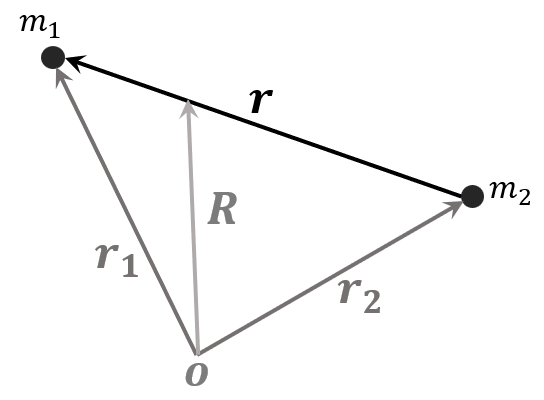
\includegraphics[width=\linewidth]{fig/fig_right.PNG}
\end{center}
\vspace*{-5mm}
\caption{二原子分子の核子の座標. }
\label{fig:phys2_fig1}
\end{figure}


$V(r)$が既知であるとして核子の波動方程式に着目する. 図\ref{fig:phys2_fig1}のように核子の座標をとると, 核子の波動方程式は, 
\begin{align}
  \label{eq:phys2_shro}
&\left( - \frac{\hbar^2}{2 m_1} \nabla_{1}^2  - \frac{\hbar^2}{2 m_2} \nabla_{2}^2 + V(r) \right) \psi(\boldsymbol{r}_1, \boldsymbol{r}_2) \nonumber \\
&= E \psi(\boldsymbol{r}_1, \boldsymbol{r}_2)
\end{align}
と書ける. $\boldsymbol{r}_1$, $\boldsymbol{r}_2$は核子1, 2の位置ベクトルであり, 核子間の距離は$r = |\boldsymbol{r}_1 - \boldsymbol{r}_2|$と表される. また$\nabla_{1}^2$, $\nabla_{2}^2$は核子1, 2のラプラシアン, $\hbar$は, プランク定数を$h$として$\hbar = \dfrac{h}{2 \pi}$, $E$は核子の波動方程式のエネルギー固有値, $\psi(\boldsymbol{r}_1, \boldsymbol{r}_2)$は核子の波動関数である. 式(\ref{eq:phys2_shro})を解くことで核子の振動・回転遷移を考える. 


核子の重心座標
$  \boldsymbol{R} = \displaystyle{\frac{m_1 \boldsymbol{r}_1 + m_2 \boldsymbol{r}_2}{m_1 + m_2} }$
と相対座標
$\boldsymbol{r} = \boldsymbol{r}_1 - \boldsymbol{r}_2$を定義し, $\boldsymbol{r}_1, \boldsymbol{r}_2, \boldsymbol{R}$  換算質量を$\mu = (m_1^{-1} + m_2^{-1})^{-1}$, 総質量を$M = m_1 + m_2$とすると重心座標・相対座標で書かれた波動方程式は
\begin{align}
\label{eq:com_each}
\left( - \frac{\hbar^2}{2 \mu} \nabla_{r}^2  - \frac{\hbar^2}{2 M} \nabla_{R}^2 + V(r) \right) \psi(\boldsymbol{r},\boldsymbol{R}) = E \psi(\boldsymbol{r},\boldsymbol{R})
\end{align}
となる。ここに
重心座標のラプラシアン
$\nabla^2_{R} = \displaystyle{\frac{\partial^2}{\partial X^2} +  \frac{\partial^2}{\partial Y^2} +  \frac{\partial^2}{\partial Z^2}}$
と相対座標のラプラシアン
$\nabla^2_{r} = \displaystyle{\frac{\partial^2}{\partial x^2} +  \frac{\partial^2}{\partial y^2} +  \frac{\partial^2}{\partial z^2}}$
を定義した。

\begin{itembox}{$\clubsuit$式{(\ref{eq:com_each}) $\,^\dagger$}}
%\tiny
\footnotesize
$\boldsymbol{R}, \boldsymbol{r}$の三次元直交座標系の第一成分を
$X, x$, 第二成分を$Y, y$, 第三成分を$Z, z$とする. 
$x$,$X$座標の変換は
\begin{align}
  x &= x_1 - x_2, 
  X = \frac{m_1 x_1 + m_2 x_2}{M} \nonumber 
\end{align}
であるから
\begin{eqnarray}
  \frac{\partial}{\partial x_1} &=& \frac{\partial x}{\partial x_1} \frac{\partial}{\partial x} +
  \frac{\partial X}{\partial x_1} \frac{\partial}{\partial X} =  \frac{\partial}{\partial x} +  \frac{m_1}{M}\frac{\partial}{\partial X}
\end{eqnarray}
より
\begin{align}
    \label{eq:x1}
  \frac{1}{m_1}\frac{\partial^2}{\partial x_1^2} =
  \frac{1}{m_1} \frac{\partial^2}{\partial x^2} + \frac{m_1}{M^2} \frac{\partial^2}{\partial X^2}
   + \frac{2}{M}\frac{\partial}{\partial x}\frac{\partial}{\partial X} 
\end{align}
また
\begin{eqnarray}
  \frac{\partial}{\partial x_2} &=& \frac{\partial x}{\partial x_2} \frac{\partial}{\partial x} +
  \frac{\partial X}{\partial x_2} \frac{\partial}{\partial X} =  - \frac{\partial}{\partial x} +  \frac{m_2}{M}\frac{\partial}{\partial X}
\end{eqnarray}
より
\begin{align}
  \label{eq:x2}
  \frac{1}{m_2}\frac{\partial^2}{\partial x_2^2} =
  \frac{1}{m_2} \frac{\partial^2}{\partial x^2} + \frac{m_2}{M^2} \frac{\partial^2}{\partial X^2}
   - \frac{2}{M}\frac{\partial}{\partial x}\frac{\partial}{\partial X} 
\end{align}

(\ref{eq:x1}, \ref{eq:x2})より
\begin{align}
 \frac{1}{m_1} \frac{\partial^2}{\partial x_1^2} +  \frac{1}{m_2} \frac{\partial^2}{\partial x_2^2} =
  \frac{1}{\mu}\frac{\partial^2}{\partial x^2} + \frac{1}{M}\frac{\partial^2}{\partial X^2}
\end{align}
同様に
\begin{align}
 \frac{1}{m_1} \frac{\partial^2}{\partial y_1^2} +  \frac{1}{m_2} \frac{\partial^2}{\partial y_2^2} &=
  \frac{1}{\mu}\frac{\partial^2}{\partial y^2} + \frac{1}{M}\frac{\partial^2}{\partial Y^2} \\
 \frac{1}{m_1} \frac{\partial^2}{\partial z_1^2} +  \frac{1}{m_2} \frac{\partial^2}{\partial z_2^2} &=
  \frac{1}{\mu}\frac{\partial^2}{\partial z^2} + \frac{1}{M}\frac{\partial^2}{\partial Z^2}
\end{align}
を足して$- \hbar^2/2$をかけると、
\begin{align}
 - \frac{\hbar^2}{2 m_1} \nabla_{1}^2  - \frac{\hbar^2}{2 m_2} \nabla_{2}^2 
= - \frac{\hbar^2}{2 \mu} \nabla_{r}^2  - \frac{\hbar^2}{2 M} \nabla_{R}^2 
\end{align}
となる。
\end{itembox}




波動方程式(\ref{eq:com_each})に対し, 波動関数$\psi(\boldsymbol{R},\boldsymbol{r})$を重心運動の波動関数$\Phi(\boldsymbol{R})$と相対運動の波動関数$\phi(\boldsymbol{r})$および重心運動のエネルギー固有値$E_R$, 相対運動のエネルギー固有値$E_r$を用いて, $\psi(\boldsymbol{R},\boldsymbol{r}) = \Phi(\boldsymbol{R})\phi(\boldsymbol{r})$, $E = E_R + E_r$と変数分離を行う. 重心運動の波動方程式と相対運動の波動方程式をそれぞれ求める。
\begin{align}
  &\Phi(\boldsymbol{R}) \left( - \frac{\hbar^2}{2 \mu} \nabla_{\boldsymbol{r}}^2 \phi(\boldsymbol{r})  + V(r) \phi(\boldsymbol{r}) - E_r \phi(\boldsymbol{r})  \right) \nonumber \\
  &+ \phi(\boldsymbol{r}) \left(  - \frac{\hbar^2}{2 M} \nabla_{\boldsymbol{R}}^2 \Phi(\boldsymbol{R}) - E_R \Phi(\boldsymbol{R}) \right) = 0
\end{align}
と変形できるので重心運動の波動方程式と相対運動の波動方程式としてそれぞれ
\begin{align}
 - \frac{\hbar^2}{2 M} \nabla_{\boldsymbol{R}}^2 \Phi(\boldsymbol{R}) &= E_R \Phi(\boldsymbol{R}) \\
- \frac{\hbar^2}{2 \mu} \nabla_{\boldsymbol{r}}^2 \phi(\boldsymbol{r})  + V(r) \phi(\boldsymbol{r}) &= E_r \phi(\boldsymbol{r}) 
\end{align}
を得る。重心運動の波動方程式は分子自体の運動を表していて、例えば平面波解が対応する。

次に相対運動の波動方程式に対し, 極座標($r, \varphi, \theta$)を用いて
  \begin{eqnarray}
    \label{eq:rotvib}
    \phi(\boldsymbol{r}) = \frac{\phi_r(r)}{r} Y(\varphi, \theta)
  \end{eqnarray}
  のように変数分離を行う. $\phi_r(r)$に対する動径方向$r$の波動方程式は, 回転による遠心力項を$W(r)$として,  有効ポテンシャル$V_\mathrm{eff} (r) = V(r) + W(r)$中を一次元運動する波動方程式に帰着する. $W(r)$を求めよう。

ラプラシアンの極座標表示は、$\nabla^2_{r, \varphi, \theta}$は, 
  \begin{align}
    \nabla^2_{r, \varphi, \theta} &= \frac{1}{r^2} \left( \frac{\partial}{\partial r} r^2 \frac{\partial}{\partial r} + \nabla^2_{\varphi, \theta} \right) \\
          \nabla^2_{\varphi, \theta} &= \frac{1}{\sin{\theta}}\frac{\partial}{\partial \theta}
        \left( \sin{\theta} \frac{\partial}{\partial \theta} \right)
        + \frac{1}{\sin^2 \theta} \frac{\partial^2}{\partial \varphi^2}
\end{align}
で与えられ、球面調和関数$Y_{lm} (\varphi, \theta)$は  
      \begin{eqnarray}
        \nabla^2_{\varphi, \theta} Y_{lm}(\varphi, \theta) + J(J+1) Y_{lm}(\varphi, \theta) = 0 
      \end{eqnarray}
を満たす. ここで$J$は回転量子数$J=0, 1, 2, \cdots$であり, $m$は$|m| \le l$を満たす整数である. 


式(\ref{eq:rotvib})を相対運動の波動方程式に代入し、ラプラシアンを極座標に変換すると
\begin{align}
  &- \frac{\hbar^2}{2 \mu} \left( \frac{1}{r^2} \frac{\partial }{\partial r} r^2 \frac{\partial }{\partial r} + \frac{1}{r^2} \nabla^2_{\varphi,\theta} \right) \frac{\phi_r(r)}{r} Y(\varphi, \theta) \nonumber \\
&+ V(r) \frac{\phi_r(r)}{r} Y(\varphi, \theta) = E_r \frac{\phi_r(r)}{r} Y(\varphi, \theta)
\end{align}
となるが、これを変数分離すると
\begin{align}
\label{eq:separation_vari}
&\frac{r^2}{ \phi_r(r)}\frac{\partial^2}{\partial r^2} \phi_r(r) + \frac{2 \mu r^2}{\hbar^2} (E_r - V(r)) \nonumber \\
&= - \frac{\nabla^2_{\varphi,\theta} Y(\varphi,\theta)}{Y(\varphi,\theta)}
\end{align}
となるから、これを$J(J+1)$と置くことで$Y(\varphi,\theta) = Y_{lm}(\varphi,\theta) $とおくことができる。

\begin{itembox}{$\clubsuit$ 式(\ref{eq:separation_vari}) $\,^\dagger$}
%\tiny
\footnotesize
\begin{align}
  &\frac{\partial}{\partial r} \left(r^2 \frac{\partial}{\partial r} \frac{\phi_r}{r} \right)
  = \frac{\partial}{\partial r} \left( r^2 \frac{r \phi_r^\prime - \phi_r}{r^2}\right) \nonumber \\
  &= \frac{\partial}{\partial r} ( r \phi_r^\prime - \phi_r)
  = \phi_r^\prime + r \phi_r^{\prime\prime} - \phi_r^\prime \nonumber \\ 
  &= r \frac{\partial^2}{\partial r^2} \phi_r(r)
\end{align}
\end{itembox}

すると動径方向の波動方程式は
\begin{align}
&- \frac{\hbar^2}{2 \mu} \frac{\partial^2}{\partial r^2} \phi_r(r) + \left(  V(r) + \frac{\hbar^2 J(J+1)}{2 \mu r^2} \right) \phi_r(r) \nonumber \\
&= E_r \phi_r(r)
\end{align}
が得られ、これは
\begin{align}
V_\mathrm{eff} (r) = V(r) + \frac{\hbar^2 J(J+1)}{2 \mu r^2} 
\end{align}
とした有効ポテンシャル中の一次元の運動とみなすことができる。よって
\begin{align}
  W(r) = \frac{\hbar^2 J(J+1)}{2 \mu r^2} 
\end{align}
となる。 

%      \begin{eqnarray}
%        \left( - \frac{\hbar^2}{2 m} \frac{d^2}{d q^2} + \frac{1}{2} m \omega^2 q^2 \right) f(q) = E^\prime f(q)
%      \end{eqnarray}

\begin{figure*}
    \centering
    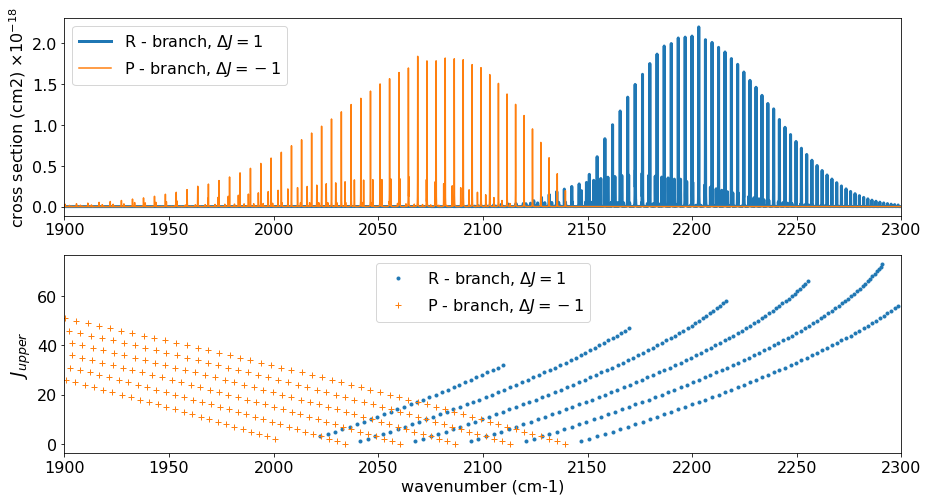
\includegraphics[width=\linewidth]{fig/branch_13_0.png}
    \caption{一酸化炭素の$\Delta \nu=1$遷移におけるR-branch, P-branch断面積。}
    \label{fig:rpbranchco}
\end{figure*}


相対運動のエネルギー固有値$E_r$について, 振動量子数$\nu$と回転量子数$J$の組を用いて, 量子状態を$(\nu,J)$で表記し, 始状態を$(\nu,J) = (\nu_i, J_i)$, 終状態を$(\nu,J) = (\nu_f, J_f)$とする.一酸化炭素のような二原子分子でみられる, $\Delta \nu = \nu_f - \nu_i = 1$, $\Delta J = J_f - J_i = \pm 1$の遷移を考える. 始状態, 終状態の相対運動のエネルギー固有値をそれぞれ$E_r = E_{r, i}$, $E_r = E_{r, f}$と表記し, 遷移エネルギーを$\Delta E = E_{r, f} - E_{r, i}$とする.  

$q=r - r_e$と座標変換する.
\begin{align}
\label{eq:vpotent}
V_\mathrm{eff} (q) &\approx V_e + \frac{\mu}{2} \omega^2 q^2 + \frac{\hbar^2 J(J+1)}{2 \mu (q + r_e)^2} \\
 &\approx V_e + \frac{\mu}{2} \omega^2 q^2 + \frac{\hbar^2 J(J+1)}{2 \mu  r_e^2} 
\end{align}
となるから$\phi_r(x)$に対する波動方程式は
\begin{align}
  &- \frac{\hbar^2}{2 \mu} \frac{\partial^2}{\partial q^2} \phi_r(q) + \frac{\mu}{2} \omega^2 q^2 \phi_r(q) = E^\prime_r \phi_r(q) \\
  &E^\prime = E_r - V_e - \frac{\hbar^2 J(J+1)}{2 \mu r_e^2}
\end{align}
と調和振動子の波動方程式となる。角振動数$\omega$の調和振動子のエネルギー固有値は, $\nu=0, 1, 2, \cdots$を振動量子数として, 
\begin{align}
  E^\prime = \hbar \omega \left( \nu + \frac{1}{2} \right) 
\end{align}
であることから, 元の波動方程式のエネルギー固有値は
\begin{align}
E_r = V_e + \hbar \omega \left( \nu + \frac{1}{2} \right) + \frac{\hbar^2 J(J+1)}{2 \mu r_e^2}
\end{align}
となる。


\begin{align}
E_r(\nu,J) = V_e + \hbar \omega \left( \nu + \frac{1}{2} \right) + \frac{\hbar^2 J(J+1)}{2 \mu r_e^2}
\end{align}
とおく。$E_{r,f} = E(\nu_f, J_f)$, $E_{r,i}=E(\nu_i,J_i)$とおけるため
\begin{align}
  \Delta E &= E_{r,f} - E_{r,i} = E(\nu_f, J_f) - E(\nu_i,J_i) \\
  &= \hbar (\nu_f -\nu_i) + \frac{\hbar^2}{2 \mu r_e^2} [J_f(J_f+1) - J_i(J_i+1)] \\
  &= \hbar \Delta \nu + \frac{\hbar^2}{2 \mu r_e^2} (J_f-J_i)(J_f + J_i + 1) \\
  \label{eq:nl}
  &= \hbar \Delta \nu + \frac{\hbar^2}{2 \mu r_e^2} \Delta J (2 J_i + \Delta J + 1)
\end{align}
となる。


$\Delta \nu = 1$, $\Delta J = 1$を式(\ref{eq:nl})に代入すると
\begin{align}
\label{eq:rbranch}
\Delta E = \hbar \omega + \frac{\hbar^2}{\mu r_e^2} (1 + J_i)
\end{align}
となる。$\Delta \nu = 1$, $\Delta J = -1$を式(\ref{eq:nl})に代入すると
\begin{align}
\label{eq:pbranch}
\Delta E = \hbar \omega - \frac{\hbar^2}{\mu r_e^2} J_i
\end{align}
となる。

これらの帰結は$\hbar \omega$を中心に前後に間隔$\frac{\hbar^2}{\mu r_e^2}$で櫛状に遷移が並ぶということである。図\ref{fig:rpbranchco}はCO ($\Delta \nu =1$)の断面積を示しており、櫛状に並んでいる。波数で右側に伸びる式(\ref{eq:rbranch})の系列をR-branch, 式(\ref{eq:pbranch})をP-branchという。


\section{ラインプロファイルと線強度}

量子力学的効果により分子の遷移エネルギーは離散的であるが、吸収エネルギーは、その離散エネルギーの周りに様々な理由で拡がる。この拡がりをBroadeningと呼ぶ。惑星大気では
\begin{itemize}
    \item 熱運動や乱流によるドップラー拡がり
    \item 不確定性原理による自然拡がり
    \item 分子間のファンデルワールス力に由来する圧力依存の圧力拡がり
\end{itemize}
の三種が重要なBroadeningである。

まず、熱運動によるbroadeningは、原子が熱運動により視線方向に速度$v_x$を持つことでおこるドップラーシフト$\nu = \hat{\nu} ( 1 + v_x/c)$に起因する。$v_x$の分布関数はMaxwell速度分布
\begin{align}
P(v_x) &= \sqrt{\frac{m}{2 \pi k_B T}} \, e^{-\frac{m v_x^2}{2 k_B T}} \\
&= \sqrt{\frac{m}{2 \pi k_B T}} \, e^{-\frac{m c^2 (\nu - \hat{\nu})^2}{2 k_B T \hat{\nu}^2}} 
\label{eq:dopplerveldist}
\end{align}
に比例してラインが広がること。HWHM (half width at half maximum)、
\begin{eqnarray}
\gamma_D = \hat{\nu} \sqrt{\frac{2 (\log{2}) k_B T}{m c^2}}
\label{eq:dopplergamma}
\end{eqnarray}
を用いて、ドップラー拡がりのline profileは
\begin{eqnarray}
g_D(\nu; \hat{\nu}; \gamma_D) = \sqrt{\frac{\log{2}}{\pi}} \frac{1}{\gamma_D} e^{ - \log{2} \left( \frac{\nu - \hat{\nu}}{\gamma_D}\right)^2}
\label{eq:dopplerprofile}
\end{eqnarray}
となる。すなわちドップラー拡がりはガウス分布に従う。乱流(ミクロ乱流)による速度分散も同様にガウス分布で近似されるが、現在のところあまり考慮されていない。

一方、圧力広がりと自然拡がりは共にLorentz profile、
\begin{eqnarray}
g_L(\nu; \hat{\nu}; \gamma_L) &=& \frac{\gamma_L/\pi}{(\nu - \hat{\nu})^2  + \gamma_L^2}
\label{eq:lorentzprofile}
\end{eqnarray}
で表される。ここにHWHMを$\gamma_L$としている。

惑星大気では特に圧力拡がり (van der Waals Broadening)が重要である。地球大気の場合、$p_0=$1 atmosphere、$T_0=$296 Kでの$\gamma_{L, \mathrm{W}}$を、air-broadening coefficient $\gamma_{L, \mathrm{W}}^{\mathrm{air}}$ といい、これを用いて、
\begin{eqnarray}
\gamma_{L, \mathrm{W}}(p,T) = \gamma_{L, \mathrm{W}}^{\mathrm{air}} \frac{p}{p_0} \left( \frac{T_0}{T} \right)^\alpha
\label{eq:airtogen}
\end{eqnarray}
のように圧力拡がりを計算することが多い。ここに$\alpha$は温度依存項のべき(temperature exponent)で代表的には0.5程度であるがさまざまである。圧力拡がりは周囲の分子からのファンデルワールス力に起因するので、背景大気の種類によって異なる。特に系外惑星大気では水素分子・ヘリウム大気であることが多く、地球の大気下での値と異なることに注意が必要である。


自然拡がりは、不確定性原理からくるラインの広がりである。アインシュタイン$A$係数を用いて
\begin{eqnarray}
\gamma_{L, \mathrm{n}} = \frac{A}{4 \pi c} = \frac{0.222}{4 \pi c} \left( \frac{\nu}{\mathrm{cm^{-1}}} \right)^2 \mathrm{[cm^{-1}]}
\end{eqnarray}
となる。これは電子が励起状態に滞在する確率が$e^{-A t}$のようになることと不確定性関係に由来している。圧力拡がりに対し、自然拡がりは低圧下で寄与が大きくなる。

上記のDoppler profileとLorentz profileの両方が効く場合、両者をconvolutionしたものがline profileとなる。これをVoigt profile\index{Voigt profile@Voigt profile}と呼ぶ。
\begin{align}
&g_V(\nu;\hat{\nu}) = ( g_L \ast g_D )(\nu; \hat{\nu}) \nonumber \\ &= \int_{-\infty}^\infty d \nu^\prime g_L(\nu - \nu^\prime;\hat{\nu};\gamma_L) g_D(\nu^\prime - \hat{\nu};\hat{\nu};\gamma_D) 
\label{eq:voigt}
\end{align}
となる。圧力拡がりと自然拡がりの両方が寄与する場合は、$\gamma_L$として
\begin{eqnarray}
\label{eq:sumgamma}
\gamma_L &=& \gamma_{L, \mathrm{W}} + \gamma_{L, \mathrm{n}}
\end{eqnarray}
を用いれば良い。これはLorentian同士の畳み込みが
\begin{align}
&g_L(\nu;\hat{\nu},\gamma_{L,\mathrm{W}}) \ast g_L(\nu;\hat{\nu},\gamma_{L,\mathrm{n}}) \nonumber \\ &= \int_\infty^\infty d \nu^\prime g_L(\nu - \nu^\prime;\hat{\nu};\gamma_{L,\mathrm{W}}) g_L(\nu^\prime - \hat{\nu};\hat{\nu};\gamma_{L,\mathrm{n}}) \\
&= \frac{(\gamma_{L,\mathrm{W}}+\gamma_{L,\mathrm{n}})/\pi}{(\nu - \hat{\nu})^2  + (\gamma_{L,\mathrm{W}}+\gamma_{L,\mathrm{n}})^2} \nonumber \\
&= g_L(\nu;\hat{\nu},\gamma_{L,\mathrm{W}}+\gamma_{L,\mathrm{n}})
\label{eq:voigt2}
\end{align}
となるからである。またLorentianのテイルは無限に続くわけではなくある程度、線中心から離れると($O(10^2) \mathrm{cm^{-1}}$)急激にカットオフが効くとされている。このSub--Lorentian効果についてはわかってないことが多いが、広い波数域で計算する際には注意が必要である。


またラインプロファイルは
\begin{align}
    \int d \nu g(\nu) = 1 
\end{align}
に規格化されているため$g(\nu)$の次元は$\mathrm{cm}$である。

光子が分子によって吸収される過程を考える。分子分光では、エネルギーに対応する量を$hc$で割って、波数で表すことが一般的である。ここでもこの表記法に習おう。また、光の吸収を考えるので、終状態は始状態より高いエネルギーである。そこで終状態を$\mathrm{up}$ (upper state)は初期状態を$\mathrm{low}$ (lower state)のラベルに書き換える。
例えば、$E_\mathrm{low} = E_{\nu_i, J_i}/hc$, $E_\mathrm{up} = E_{\nu_f, J_f}/hc$である。

光の吸収に関して各ラインの強度は、下の順位$E_\mathrm{low} $からの誘導吸収により生じるため、その状態の数に比例して強くなる。ただし、光が入射することで生じる誘導放射により実効的な吸収が減るため、この補正も必要である。

$E_\mathrm{low}$の状態の数は、局所熱力学平衡にあると
\begin{align}
\label{eq:lte}
    \frac{n_\mathrm{low}}{n} &= \frac{\mathsf{g}_\mathrm{low}}{Q(T)} \exp{\left(- \frac{h c E_\mathrm{low}}{k_B T} \right)}
\end{align}
となる。ここに$\mathsf{g}_\mathrm{low}$は縮退度、$n$は全状態数、$Q(T)$は分配関数である。また誘導放射による補正は$(1- e^{-h c \hat{\nu}/k_B T})$である。ここに$\hat{\nu}$は吸収波数、つまりupper/lower statesの差の$\hat{\nu} = E_\mathrm{up} - E_\mathrm{low}$のことである\footnote{この量を$E$を使って表さないのは、分光的に問題となる実際に吸収中心である波数であるからであろう。}。

係数も含めると線強度とはラインプロファイル$g(\nu)$を用いて断面積が
\begin{align}
    \sigma^2 (\nu) = S(T) g(\nu)
\end{align}
となる量である。つまり$S(T)$の次元は$\mathrm{cm}$である。

\begin{align}
\label{eq:STexomol}
S(T) &=\displaystyle{ \frac{\mathsf{g}_\mathrm{up}}{Q(T)} \frac{ A}{8 \pi c \hat{\nu}^2} e^{-  c_2 E_\mathrm{low}/T} {\left(1- e^{-c_2 \tilde{\nu}/T}\right)}},
\end{align}
となる。ただし$c_2 \equiv hc/k_B = 1.4387773 \, \mathrm{cm K}$である。$A$はアインシュタインA係数である。

\begin{itembox}{$\clubsuit$ 式(\ref{eq:STexomol}) $\,^\dagger$}
%\tiny
\footnotesize
実効的に起きる吸収は、誘導吸収($B_{lu}$)から誘導放射($B_{ul}$)を差し引いたものである。つまり
\begin{align}
    S(T) &= \frac{h c \hat{\nu}}{c} \left( \frac{n_\mathrm{low}}{n} B_{lu} - \frac{n_\mathrm{up}}{n} B_{ul} \right) 
\end{align}
が実効的におこる吸収である。局所熱力学平衡の場合、
\begin{align}
     \frac{n_\mathrm{up}}{n_\mathrm{low}} &= \frac{\mathsf{g}_\mathrm{up}}{\mathsf{g}_\mathrm{low}} \exp{\left(- \frac{h c (E_\mathrm{up} - E_\mathrm{low})}{k_B T} \right)} \\
     &= \frac{\mathsf{g}_\mathrm{up}}{\mathsf{g}_\mathrm{low}} e^{-hc \hat{\nu}/k_B T}
\end{align}
である。また詳細つり合いから
\begin{align}
    \mathsf{g}_\mathrm{low} B_{lu} &= \mathsf{g}_\mathrm{up} B_{ul} \\
    A &= 2 \pi h c \hat{\nu}^3 B_{ul}
\end{align}
となるが、これらを用いると
\begin{align}
    S(T) &= \frac{h \hat{\nu}}{4 \pi} \frac{n_\mathrm{low}}{n} B_{lu} (1 -  e^{-hc \hat{\nu}/k_B T}) \\
    &= \frac{\mathsf{g}_\mathrm{up}}{Q(T)} \frac{ A}{8 \pi c \hat{\nu}^2} e^{- h c E_\mathrm{low}/k_B T} {\left(1- e^{- h c \tilde{\nu}/k_B T}\right)}
\end{align}
が得られる。途中で式(\ref{eq:lte})を用いた。
\end{itembox}



\section{様々な分子の振動回転遷移$^\ddagger$}
\subsection*{メタン}
%https://doi.org/10.1016/j.jqsrt.2024.108897

\begin{figure}
    \centering
    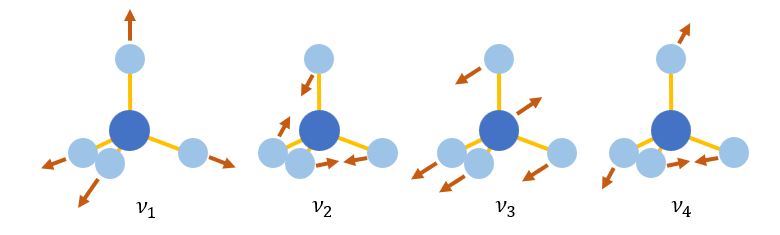
\includegraphics[width=\linewidth]{fig/methanevib.png}
    \caption{メタンの4種振動モード}
    \label{fig:ch4vib}
\end{figure}

図\ref{fig:ch4vib}に示すように、メタンの振動モードは4種類$\nu_1, \nu_2, \nu_3, \nu_4$があり、そのうち赤外活性つまり赤外域での光子吸収があるのは$\nu_3$と$\nu_4$である。これらは基本バンドとして、それぞれ3.25--3.45 $\mu$m, 7.5--8.0$\mu$mに強い吸収を持つ。またそれ以外の場所にもPolyad構造による吸収(ホットバンド)が多数存在する。Polyad構造は
$\nu_1 \simeq \nu_3 \simeq 2 \nu_2 \simeq 2 \nu_4 \simeq 3000\mathrm{cm}^{-1}$ となることに起因する構造であり、polyad数
\begin{align}
\mathrm{P} =  2 (\nu_1 + \nu_3) + \nu_2 + \nu_4 
\end{align}
で特徴づけられる。それぞれ
Monad (P=0),
Dyad (P=1),
Pentad (P=2),
Octad (P=3),
Tetradecad (P=4),
Icosad (P=5),
Triacontad (P=6),
Tetracontad (P=7),
の名前がついていて、エネルギーは大まかに$1500 P \mathrm{cm}^-1$程度となる。例えば褐色矮星のHバンドに見られる1.6$\mu$m付近のメタン吸収はP=4のTetradecadに対応することが分かる\cite{2024JQSRT.31608897K}。\\


\subsection*{二原子分子のバンドヘッド}

調和振動子近似ではポテンシャルが核子間距離の二次の関数であるとし、式(\ref{eq:vpotent})の遠心力項が核子間の距離の関数であることを無視していた。実際、この近似は、図\ref{fig:rpbranchco}のように、一酸化炭素の$\Delta \nu=1$遷移をよく説明できる。
しかし、振動遷移$\Delta \nu$が大きくなってきて核子間距離の、これらの近似が破れてきて、バンドヘッドという構造が表れる。ポテンシャルは
\begin{align}
\label{eq:vpotent_}
V_\mathrm{eff} (q) &\approx V_e + \frac{\mu}{2} \omega^2 q^2 + \frac{\hbar^2 J(J+1)}{2 \mu r_e^2 [1 + (q/r_e)^2]} \\
&\approx \frac{\hbar^2 J (J+1)}{2 \mu r_e^2} \left[1 - 2 \frac{q}{r_e} + 3 \left(\frac{q}{r_e} \right)^2 \cdots + \right]
\end{align}
と表されるが、この右辺第三項の$q/r_e$が大きくなると、遠心力が弱くなる効果が存在する。また、ポテンシャル自身も図\ref{fig:co_ele_state}の基底状態で示すように平衡位置から離れると二次近似から逸脱してくる。これらの効果を摂動論として計算すると、(省略するが)この計算は$X=(\nu + 1/2)$と$Y=J(J+1)$の二次式の形となる。

クロスターム($XY$)以外の二次の項は無視した形式を記すと
\begin{align}
    \label{eq:nonharmo_cen}
    E_r (\nu, J) &= V_e + \hbar \omega \left( \nu + \frac{1}{2} \right) + B_\nu J (J+1)  \\
    \label{eq:nonharmo_cen_x}
    B_\nu &= \frac{\hbar^2}{2 \mu r_e^2} - \alpha_0  \left( \nu + \frac{1}{2} \right) 
\end{align}
となる。これは振動が大きくなると、非調和ポテンシャルでは平均的な核間距離が延びることで、回転定数$B_\nu$が小さくなるという描像である。

式(\ref{eq:nonharmo_cen_x})を用いて評価すると $B_{\nu+1} - B_\nu = - \alpha_0$であるので、R, P-branchはそれぞれ
\begin{align}
\label{eq:u_fort_R}
    h \hat{\nu}^R_{\mathrm{line}} (J_u) &= h \nu_\nu  + 2 B J_u - \alpha_0 J_u^2  \\
\label{eq:u_fort_P}
    h \hat{\nu}^P_{\mathrm{line}} (J_u) &=  h \nu_\nu - 2 B (J_u + 1) - \alpha_0 (J_u + 1)^2 \\
    B &\equiv B_0 + \frac{1}{2} \alpha_0
\end{align}
となり二次関数となる。

$\alpha_0 > 0$とすると、R-branchの変曲点は$J_u = B/\alpha_0 > 0$となるので\footnote{一方、P-branchの変曲点は$- B/\alpha_0 < 0$であるので、$J_l = J_u+1 > 0$の領域に変曲点は存在しない。ただしこれは$\alpha_0>0$の場合である。}、振動回転遷移の波数最大値(波長最小値)が存在し、このエネルギー付近に多数の遷移が集まることがわかる(図\ref{fig:rpbranch}の下パネル)。これをband headと呼ぶ。図\ref{fig:rpbranch}に2.3ミクロン付近のCOのband headの例を示した。今回横軸は波長であることに注意が必要である。band head付近の準位が多い温度では、band head付近の吸収が強くなる(図\ref{fig:rpbranch}の上パネル)。

\begin{figure*}
    \centering
    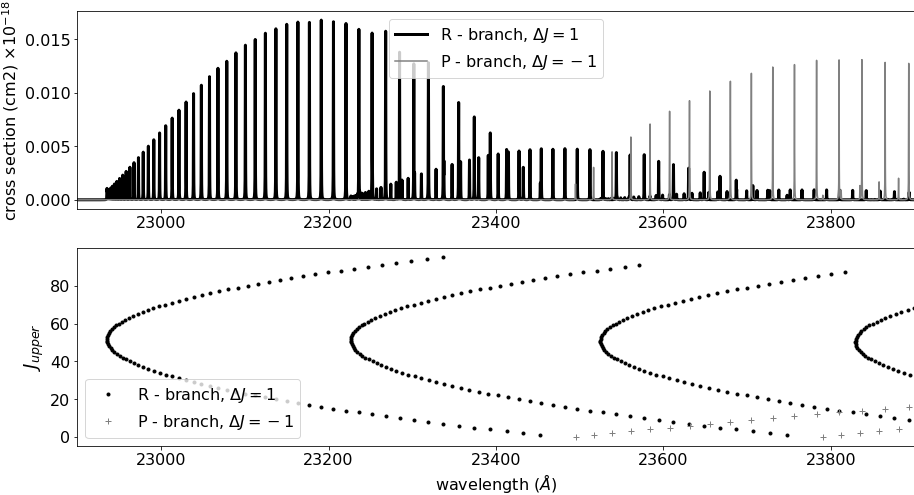
\includegraphics[width=0.9\linewidth]{fig/bandhead.png}
    \caption{CO 2.3ミクロン帯 ($X\,^1 \Sigma^+$, $\Delta \nu = 2$)のband headの例。$J_{upper}$のエネルギー増加が減少に転じる点に多数の遷移が集まりband headが生じる。}
    \label{fig:rpbranch}
\end{figure*}



また式(\ref{eq:u_fort_R})と(\ref{eq:u_fort_P})を一つの式にまとめて、
\begin{align}
    h \hat{\nu}_{\mathrm{line}} (\mathcal{J}) &=  h \nu_\nu - 2 B \mathcal{J} - \alpha_0 \mathcal{J}^2 
\end{align}
ただし、
\begin{align}
    \mathcal{J} = \left\{
\begin{array}{ll}
J_u & (\mathcal{J} > 0)\\
- J_l & (\mathcal{J} < 0)
\end{array}
\right.
\end{align}
としたものを、縦軸$\mathcal{J}$、横軸ライン中心波数で書いたものを
R. Fortratにちなんでフォルトラ図という(図\ref{fig:fortrat})。振動エネルギーの差にあたる$\mathcal{J}=0$の値$\nu_\nu$にはラインがない。これをバンド原点(Band origin)と呼ぶ。

\begin{figure*}
    \centering
    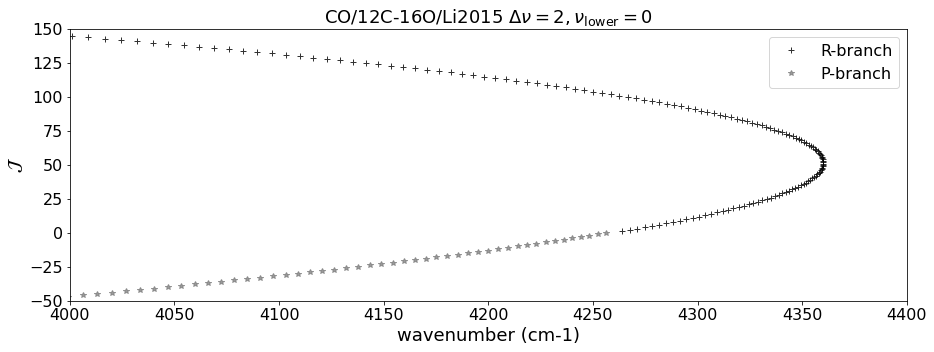
\includegraphics[width=0.9\linewidth]{fig/fortrat.png}
    \caption{COのフォルトラ図。$\Delta \nu=2$, $\nu_\mathrm{lower}=0$の場合を示している。}
    % exojax/documents/tutorials/Fortrat.ipynb
    \label{fig:fortrat}
\end{figure*}
